\chapter{HTML简介}

\section{前后端}

\subsection{前端工程师(Front-End Engineer)}

前端工程师互联网时代软件产品研发中不可缺少的一种专业研发角色。前端是一个相对比较新的行业,大约从2005年开始,正式的前端工程师角色被行业所认可。到了2010年,互联网开始全面进入移动时代,前端工程师的地位也越来越重要。 \\

现在一些后端开发工作也可以由前端工程师来完成。最初所有的开发工作都是由后端工程师完成的,但是随着业务越来越繁杂、工作量过大,后端工程师们不堪重负,于是将可视化和部分交互功能的开发剥离出来,形成了前端开发。 \\

前端工程师主要负责的工作就是使用HTML、CSS、JavaScript等专业技能和工具将产品UI设计稿实现成网站产品。涵盖用户PC端和移动端网页,处理视觉和交互问题。 \\

广义上讲,所有用户终端产品,只要是与视觉和交互有关的部分都是前端工程师的专业领域。产品从前期开发到后期的维护、更新、升级都需要前端工程师来完成。

\subsection{后端工程师(Back-End Engineer)}

后端工程师主要负责服务器的数据逻辑和业务逻辑等,主要研究怎么把数据更好地传输给前端工程师。 \\

如果一个人除了完成前端开发和后端开发工作以外,从产品设计到项目开发,再到后期运维都是同一个人,甚至可能还要负责UI、配动画、写文档等,那么就被称为全栈工程师(Full Stack Engineer)。

\subsection{前端应用领域}

前端技术可以被应用在一系列领域中:

\begin{itemize}
    \item 网页网站
    \item APP、微信小程序
    \item 移动端小游戏
    \item 炫酷的特效
    \item 大数据可视化
    \item VR虚拟现实
\end{itemize}

前端工程师需要具备大量必要的技能,其中前端三大基础语言为HTML、CSS、JavaScript,除此之外还需要学习jQuery、网络、es6、webpack4.0、小程序、VUE、React、Node.js、Mongo DB数据库等内容。 \\

\newpage

\section{结构层/表现层/行为层}

\subsection{结构层/表现层/行为层}

\begin{itemize}
    \item 结构层HTML(HyperText Markup Language):一个超文本标记语言,负责描绘出网页内容的架构。
    
    \item 表示层CSS(Cascading Style Sheets):层叠样式表,负责如何显示结构层的有关内容。
    
    \item 行为层JavaScript:目前在Web上使用的最主要的客户端脚本语言,是Web脚本语言的一个标准,可以对结构层和表现层的内容随意进行更改。
\end{itemize}

\subsection{代码注释}

在HTML、CSS、JavaScript中代码的注释是不一样的。

\begin{lstlisting}[style=htmlcssjs, title=HTML注释,keywordstyle=\color{brown},]
<!-- 注释内容 -->
\end{lstlisting}

\begin{lstlisting}[style=htmlcssjs, title=CSS注释]
/* 注释内容 */
\end{lstlisting}

\begin{lstlisting}[style=htmlcssjs, title=JavaScript注释]
// 注释内容
/* 注释内容 */
\end{lstlisting}

\newpage

\section{Hello World!}

\subsection{Hello World!}

问候一下世界,制作人生中的第一个HTML网页吧。

\begin{lstlisting}[style=htmlcssjs, title=Hello World!]
<!DOCTYPE html>
<html lang="en">
<head>
    <meta charset="UTF-8">
    <title>Hello World!</title>
</head>
<body>
    Hello World!
</body>
</html>
\end{lstlisting}

\subsection{HTML和CSS的关系}

先来看一下单纯的HTML标签长什么样:

\begin{figure}[H]
	\centering
	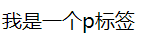
\includegraphics[]{img/C1/1-3/1.png}
\end{figure}

再来看一下经过CSS修饰过后的HTML标签:

\begin{lstlisting}[style=htmlcssjs, title=Hello World!]
p {
    color: red;
    border: 1px solid red;
    width: 140px;
    height: 40px;
}
\end{lstlisting}

\begin{figure}[H]
	\centering
	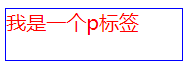
\includegraphics[]{img/C1/1-3/2.png}
\end{figure}

